\chapter{Origins of Multi-decadal Variability in Sudden Stratospheric Warming events}
\label{cha:models}
\begin{quotation}
  Much of the work presented in this chapter is based on Dimdore-Miles et al. 2020 (ref) however the analysis has been extended here to include a more comprehensive diagnosis of stratospheric variability in the UKESM gcm.
\end{quotation}


\section{Introduction}
\label{sec:origins_introduction}
Despite a significant body of work aimed at understanding the nature of vortex variability including SSWs, variations in this mode on decadal to multi-decadal timescales is not well understood. A formal diagnosis of such variability as well as a better understanding of factors which influence it may help to improve predictability of SSWs and subsequently NH mid-latitude surface climate.

Nevertheless, some studies have addressed the notion of low frequency variations in the vortex. \cite{Garfinkel2017} analyse decadal-scale variations in vortex strength in a set of historical simulations and propose that an observed hiatus in Eurasian surface warming was most likely due to variability in midwinter vortex strength. Similarly, \cite{cohen2009} find decadal scale variations in planetary wave forcing of the vortex in a suite of CMIP3 models as well as NCEP–NCAR reanalysis. Whether the vortex variability was forced by greenhouse gas concentrations or arose through internal variability in these studies was not fully established but \cite{Garfinkel2015} used a subset of the simulations analysed in \cite{Garfinkel2017} and linked a decadal trend (1980-2009) in late winter vortex strength to SST variability. On the other hand, \cite{Seviour2017} analysed observed variations between 1980 and 2016 and concluded that the vortex variability was primarily internally generated. Other studies also point towards internally generated decadal fluctuations in vortex strength: \cite{Manzini2012} explore causes of 20 year period variability in a simulation with prescribed, pre-industrial SSTs. They propose that, given the boundary conditions in the simulations are fixed, such variability must be internally generated. Finally, \cite{Butchart2000} suggest that decadal variability in vortex strength as well as SSW frequency may originate from feedbacks caused by the non linear nature of boreal winter stratospheric dynamics.

On longer timescales, \cite{Schimanke2011} noted variations in SSW occurrence with periods of approximately 52 years in a multi-century GCM integration and demonstrated coherent variability in other parts of the climate system, including vertically propagating planetary wave activity, Eurasian snow cover and Atlantic SSTs. However, despite providing some indications of externally driven variability, results from this study are not conclusive, since the GCM used (EGMAM: ECHO‐G with Middle Atmosphere Model) exhibits significant bias in mean SSW rate compared to reanalyses (2 events per decade). The authors also note that further simulations are required to understand this variability. 

multi-decadal scale variations in climate features which can couple with the vortex has also been explored. There are clear decadal variations in the period and phase transition timing of the QBO \citep{Pascoe2005,Anstey2008,Yang2016}. These may be linked to variations in the degree of 'stalling' of the QBO phase descent, which can cause more or less persistent wind direction at a given level.  A number of studies have also noted the transient nature of the strength of the HT relationship \citep{Lu2008,Lu14,Anstey2008,OspEA10}. \cite{Lu2008,Lu14} note that the mid-latitude wave-guide is modulated by the shape of the vortex so that planetary waves are diverted further equatorwards when the vortex is anomalously strong and wide, and this could temporarily reduce the influence of the QBO on the vortex. The AL also varies significantly on decadal to multi-decadal timescales. \cite{Overland1999} note that 10 year mean values of SLP over the AL region exhibit fluctuations of up to 35\% of the climatological mean. Subsequent studies corroborate the presence of these decadal scale fluctuations: \cite{SUGIMOTO2009} and \cite{Minobe} show 20 year fluctuations in intensity and centre of action of the AL while \cite{Raible2005} propose a 50-60 year trend in AL intensity, suggesting the existence of even longer timescale variability. 

\section{Data And Methods}
\subsection{Model Configuration}
For analysis of multi-decadal variability in the vortex and SSWs, we utilise a simulation of the first version of the UK Earth System Model (henceforth referred to as UKESM), the most recent configuration of the MetOffice unified model (the UM) \citep{Mulcahy2018}. UKESM is a stratosphere resolving coupled ocean-atmosphere-land-sea ice model. The Atmospheric component is GA7.1 with 85 vertical levels from the surface to 85km, 35 of which are above 18km \citep{Walters2019, Williams2018}. The model is run at N96 horizontal resolution (approximately 135 km near the equator). The ocean model used is GO6.0 \citep{Storkey2018} which contains 75 levels and runs at 1${^\circ}$ horizontal resolution. Land surface and sea-ice processes are represented by JULES \citep[GL7.0,][]{Walters2019} and CICE  \cite[GSI8.1,][]{Ridley2018} models respectively, while ocean biochemistry is added through MEDUSA \citep{Yool2013}. UKESM also includes a fully interactive chemistry scheme via coupling with the UK Chemistry and Aerosols model \citep[UKCA,][]{Mulcahy2018}.

We utilise a 1000 year pre-industrial (PI) control simulation of UKESM submitted to CMIP6 which is spun-up to achieve initial model equilibrium following the method outlined in \cite{Yool20}. This run is forced using CMIP6 pre-industrial values for concentrations of major GHGs (global mean 284.317ppm $CO_2$, 808.25ppb $CH_4$, 273.02ppb $N_2O$). While there are no volcanic eruptions in the simulation, background stratospheric volcanic aerosols are set to climatological values between 1850 and 2014 estimated from satellite products and other model simulations \citep{Menary2018}. We choose a PI control for this analysis to examine internal variability in SSWs on multi-decadal timescales. 


\subsection{Reanalysis Data}
To verify that the model reproduces relevant features of the climate system we compare with an observation based dataset produced by the ECMWF - ERA-Interim \cite{Dee2011}. The ERA-interim dataset is produced by a 4D-Var data assimilation method of a wide range of observations \citep{Uppala2005}. These include surface measurements, aircraft campaign data, radiosonde readings and satellite observations. The 4D-var data assimilation process involves supplying the ECMWF’s Integrated Forecast System (IFS) initial conditions from observations, letting the model evolve for a timestep and re-initialising for the next step with a combination of output and updated observations \citep{Courtier1998, Bouttier2001}. This update is carried out to minimise a cost function defined to capture the difference between the latest model output and observations for that corresponding time. ERA-Interim provides data on 60 vertical levels at a maximum horizontal resolution of $\sim$ 80 km from 1979-2019 \citep{Berrisford}.

The majority of observations assimilated for ERA-Interim are satellite based radiance retrievals. These are gained from nadir facing satellites which measure spectral radiances (energy detected at difference wavelengths). A single detection device will consist of several channels which detect radiation from difference wavelengths. Different atmospheric layers absorb and emit at different wavelengths so measuring over a range of channels can build up a vertical profile of temperature (for example). However, the atmospheric layers that are detected by each channel may overlap resulting in measurements from multiple channels being used in the retrieval of a given layer. A weighting is applied to the channels at each height to account for the proportion of the total measurement that should be contributed by each channel. Channel weighting profiles (figure \ref{fig:Satellite_channels}) \citep{Fujiwara17} are generally Gaussian (for Nadir Satellites) in pressure, the width of which signifying the vertical extent of the channel. The vertical resolution of the retrievals is determined by the density of channels covering a particular height range. 

During the ERA-Interim period, the set of observations used for assimilation have developed significantly. Between 1979 and 1998 only limited satellite based radiance retrievals are available to produce profiles. These satellite observations are primarily provided by the Stratosphere Sounding Unit (SSU) and Microwave Sounding Unit (MSU) which are parts of the TRIOS Operational Vertical Sounder (TOVS) suite. The SSU possesses only 3 channels (figure \ref{fig:Satellite_channels}a) and therefore provides data at relatively coarse vertical resolution. Over this period, ERA-interim relies heavily on direct measurement techniques such as radiosondes, dropsondes and aircraft \citep{Fujiwara17} which bring possible biases from the influence of shortwave solar heating on temperature sensors in radiosondes as well as warmer tendencies in aircraft based observations compared to radiosondes \citep{Ballish2008}. After 1998 more extensive satellite based measurements are available for assimilation and are incorporated in ERA-interim. The new satellite products include improved versions of the SSU and MSU as a part of the Advanced TRIOS Operational Vertical Sounder (ATOVS) suite which provides profiles derived from the Advanced Microwave Sounding Unit A (AMSU, figure \ref{fig:Satellite_channels}b) from which ERA-interim calculates profiles using 11 channels (channels 5-14 from AMSU). ERA-Interim also makes use of a number of other satellite based instruments which are fully outlined in \citep{Fujiwara17}. Possible sources of biases in these satellite based observations include orbital drift and calibration offsets \citep{Zou2006,Simmons2014}.

As a result of including additional observations for assimilation after 1998, ERA-interim shows a shift in temperature structure of the middle and upper stratosphere between the two periods. Caution is therefore, advised when using this data for trend analysis \citep{Long2017} however such an analysis does not form part of the work in this thesis. Zonal wind fields show little change across the periods. Additionally, ERA-interim struggles (as the majority of modern reanalyses do) to constrain phase transition timing of the QBO correctly \citep{Kawatani2016}. Comparisons with wind profiles derived from a single radiosonde station, Singapore at $^{\circ}$1N, $104^{\circ}$E, which covers a large majority of the reanalysis period, show that ERA-interim also exhibits biases in the amplitude of both QBO phases. These biases reduce significantly with the transition to the use of ATOVS \citep{Kawatani2016,Long2017}. Similar biases and improvements over the TOVS-ATOVS period are also observed for representation of the SAO \cite{BaldwinGray2005}. These biases must be taken into account when considering comparisons in stratospheric circulation between ERA-interim and GCMs. Nonetheless, \cite{Long2017} stress that these datasets are in broad agreement with other major reanalyses in the stratosphere and lower mesosphere.

\begin{figure}[h!]
\centering
    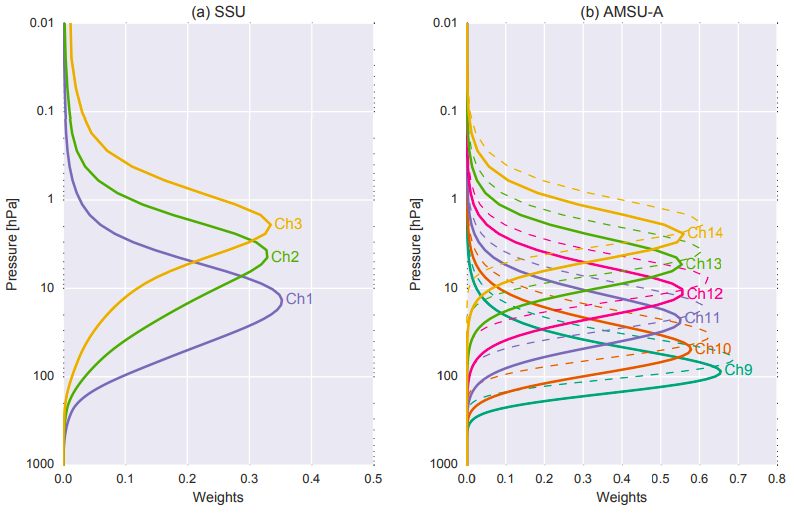
\includegraphics[width=0.5\textwidth]{Figures/Figures-origins/channels.png}
    \caption[Channel profiles for satellite retrievals assimilated by ERA-Interim]{Figure from \cite{Fujiwara17} \textbf{Left}: Channel weighting profiles for the TOVS Stratospheric Sounding Unit (SSU) used for ERA-Interim dataset in the period 1979-2005. \textbf{Right}: Weighting profiles from the ATOVS-suite Advanced Microwave Sounding Unit (AMSU) which provides measurements for ERA-Interim from 1998-present. Solid lines represent near Nadir profiles and dashed lines signify limb profiles (taken at an angle of $48.33^{\circ}$).}
    \label{fig:Satellite_channels}
\centering
\end{figure}

\subsection{Wavelet Analysis}
\label{sec:Wavelet_Analysis}
In order to study possible multi-decadal variability in SSW occurrence, we utilise a wavelet analysis method based on \cite{Torrence1998}. Such an analysis can be used to examine time series which displays non-stationary spectral power over multiple frequencies \citep{Daubechies} giving it a useful advantage over more traditional fourier methods for spectral analysis. The wavelet transform of a uniform 1-dimensional time series, $x$, of length $N$ and timestep $\delta t$ is given by the convolution between the series and a scaled and translated version of a wavelet function $\psi_0$ (equation \ref{wavelet_transform})

\begin{equation} \label{wavelet_transform}
W_n(s) = \sum^{N - 1}_{n' = 0} x_{n'} \psi^* \bigg[(n' - n) \frac{\delta t}{s}\bigg],
\end{equation}

where $*$ denotes the complex conjugate and $s$ is the wavelet scale indicating the frequency of the wavelet. Varying $s$ and translating along the time scale (the index $n$), $W_n$ indicates the amplitude of signals at different scales and their variation in time. \cite{Torrence1998} suggest an approach to varying the scale s as increasing in powers of 2 according to 

\begin{equation} \label{S}
s_j = s_0 2^{j \delta j},\\ j = 0, 1, ..., J
\end{equation}

\begin{equation} \label{S}
J = \delta j^{-1} log_2\bigg(\frac{N \delta t}{s_0}\bigg),
\end{equation}

where $s_0$ is the shortest resolvable scale of a signal, J corresponds to the longest and $\delta j$ is the scale resolution. The translated and scaled wavelet has the form

\begin{equation} \label{wavelet}
\psi^* \bigg[(n' - n) \frac{\delta t}{s}\bigg] = \bigg(\frac{\delta t}{s}\bigg)^{1/2} \psi_0\bigg[(n' - n) \frac{\delta t}{s}\bigg]
\end{equation}

and we select the form of $\psi_0$ following the recommendation of \cite{Torrence1998} as a Morlet wavelet, an oscillatory function enveloped by a Gaussian which is expressed as

\begin{equation} \label{psi0}
\psi_0(p) = \pi^{-1/4} e^{i\omega_0 p} e^{\frac{p^2}{2}}.
\end{equation}

The advantages of using a Morlet wavelet for analysing signals in climate time-series is discussed in \cite{Lau1995} in which the authors acknowledge that while truly physical signals should be detected regardless of which wavelet basis is chosen, for best results one should adopt a wavelet function reminiscent of the real signal. They show that when a Morlet wavelet form is utilised, spectral decomposition methods can detect common forms of behaviour exhibited in the variability of time series associated with the Earth's climate. These include time variations in period and amplitude of signals, abrupt changes in periodicity (sudden regime shift to different spectral behaviour) and some forms of rapid changes in series over time. These forms of behaviour are most likely relevant for our analysis of SSWs, therefore we proceed with a wavelet of this form. 

It is computationally quicker to compute the wavelet transform in discrete Fourier space. By the convolution theorem, the transform reduces to multiplication

\begin{equation} \label{wavelet_transform2}
W_n(s) = \sum^{N - 1}_{k = 0} \hat{x}_{k} \hat{\psi}^* (s\omega_k) e^{i \omega_k n \delta t},
\end{equation}

where $\hat{x}_{k}$ and $\hat{\psi}$ are the discrete Fourier transforms of the time series $x$ (equation \ref{fourier1}) and the wavelet function (equation \ref{fourier2}) respectively,

\begin{equation} \label{fourier1}
\hat{x}_k = \frac{1}{N} \sum^{N-1}_{n = 0} x_n e^{\frac{-2\pi i k n}{N}}
\end{equation}

\begin{equation} \label{fourier2}
\hat{\psi}(s\omega_k) = \bigg(\frac{2 \pi s}{\delta t}\bigg) \pi^{-1/4}H(\omega_k) e^{-(s\omega_k - \omega_0)^2/2}.
\end{equation}

$H(\omega_k)$ is the Heavyside function and $\hat{\psi}$ is normalised to have unit energy when integrated over all $\omega$. The square modulus of the wavelet transform gives the wavelet power spectrum which indicates relative strength of signals in the time series as a function of signal period and discretised time. In order to directly compare spectra of different indices we normalise all spectra by the variance of the corresponding time series. We also define a confidence interval for wavelet power observed at a given period and time for a series by assuming a mean background spectrum corresponding to that of a first order autoregressive (AR1, red noise) process modelled by

\begin{equation} \label{rednoise}
x_n = \alpha x_{n - 1} + z_n,
\end{equation}

where $\alpha$ is the lag-1 autocorrelation of the time series and $z_n$ is Gaussian white noise. \cite{Torrence1998} show that such a process's wavelet power spectrum is $\chi^2$ distributed and therefore can be used to define a 95\% confidence interval for any observed power. 

\subsection{Cross Wavelet Spectra}
The cross wavelet spectrum of two time series $x$ and $y$ with associated wavelet spectra $W^x_n$ and $W^y_n$ gives a measure of coincident power (the same period at the same timepoints) between the series. It is given by

\begin{equation} \label{wavelet_cross}
\vert W^{xy}_n(s)\vert = \vert W^{x*}_n(s) W^{y}_n(s)\vert,
\end{equation}

where $W^{x*}_n(s)$ is the complex conjugate of the wavelet power spectrum of $x$ \citep{Grinstead2004}. The complex argument of $W^{xy}_n(s)$ gives the local phase difference between signals in $x$ and $y$ in frequency-time space. The phase relationship between the two time-series can be represented by a
vector that subtends an angle representing the phase difference: On all plots of cross spectra, arrows to the right (left) denoted signals which are in-phase and correlated (anti-correlated). Vertical arrows indicate a phase relationship of $\frac{\pi}{2}$ between the time-series, so that the evolution of
one is correlated with the rate-of-change of the other. As for individual power spectra, we define a confidence interval for which cross power of a larger amplitude is deemed significant (>95\% confidence interval) by comparing power exhibited by actual series with a theoretical red noise process. The cross power of two such AR1 processes is theoretically distributed such that the probability of obtaining cross power greater than a set of red-noise processes is

\begin{equation} \label{wavelet_cross_dist}
D\bigg(\frac{\vert W^{xy}_n(s)\vert}{\sigma_x \sigma_y} < p\bigg) = \frac{Z_\nu(p)}{\nu} \sqrt{P^x_k P^y_k},
\end{equation}

where $\sigma$ denotes the standard deviation of the time series, Z is the confidence interval defined by $p$ ($Z$ = 3.999 for 95\% confidence), $\nu$ is the degrees of freedom for a real wavelet spectrum ($\nu$ = 2) and $P^x_k$ is the theoretical Fourier spectrum of the AR1 process. For a given wavenumber k, this can be expressed as

\begin{equation} \label{theoretical_fourier}
P_k = \frac{1 - \alpha^2}{\vert 1 - \alpha e^{2i\pi k} \vert^2}.
\end{equation}

\subsection{Hilbert Transform}
We utilise a signal processing method known as a Hilbert transform to calculate the instantaneous phasor amplitude of a QBO time series. The Hilbert transform of a time series $x(t)$ can be expressed as

\begin{equation} \label{theoretical_fourier}
\tilde{x} = Hil[x(t)] = \frac{1}{\pi t} * x(t),
\end{equation}

where $\tilde{}$ denotes the transformed series, * signifies a convolution and $t$ is discretised time. Conversely, the original time series can be recovered using an inverse transform expressed as

\begin{equation} \label{theoretical_fourier}
{x(t)} = Hil^{-1}[\tilde{x}(t)] = -\frac{1}{\pi t} * \tilde{x}(t).
\end{equation}

A complex signal which consists of $x(t)$ and its transform is known as the analytic signal of $x$ and can be used to calculate an instantaneous phasor amplitude, $A(t)$, of the signal. $X(t)$ can be expressed as

\begin{equation} \label{theoretical_fourier}
X(t) = x(t) + \tilde{x}(t) i = A(t) e^{i\theta},
\end{equation}

where $A(t)$ is the instantaneous amplitude of the signal and $\theta(t)$ is the instantaneous phase angle - a measure of signal progression through a cycle at time $t$.


% Re-address aims from introduction

%%% Local Variables:
%%% mode: latex
%%% TeX-master: "thesis"
%%% End:
